\section{Wyniki pomiarów działania programu}
\subsection{Dokładność modeli w bazie}
Badania przeprowadzono dla różnych liczb n-literowych końcówek wyrazów. 
\begin{landscape}
	\noindent Aby lepiej zobrazować otrzymane wyniki użyto notacji:\\ (liczba 1 literowych końcówek, liczba 2 literowych końcówek, liczba 3 literowych końcówek, liczba 4 literowych końcówek).
	\begin{table}[H]
		\centering
		\caption{Skuteczność modeli -- korpus PWr.}
		\begin{tabular}{cccccccc}
			\toprule
			\textbf{Algorytm} & \textbf{(15, 35, 35, 35)} & \textbf{(20, 35, 35, 35)} & \textbf{(25, 38, 38, 38)} & \textbf{(25, 40, 40, 40)} & \textbf{(28, 42, 42, 42)} & \textbf{(28, 45, 45, 45)} & \textbf{(32, 45, 45, 45)} \\
			\midrule
			Support Vector Machine & 56,46 & 57,46 & 58,75 & 60,03 & 61,01 & 59,94 & 58,68 \\
			Decision Trees & 57,24 & 58,12 & 59,30 & 59,97 & 60,58 & 59,10 & 58,14 \\
			Stochastic Gradient Descent & 53,62 & 54,48 & 55,37 & 56,58 & 57,72 & 56,22 & 54,97 \\
			Logistic Regression & 55,57 & 56,68 & 57,93 & 58,82 & 59,93 & 58,79 & 57,84 \\
			Naive Bayes & 54,14 & 55,42 & 56,69 & 57,72 & 58,89 & 57,58 & 56,56 \\
			K Neighbors & 50,17 & 51,35 & 52,18 & 53,30 & 54,22 & 53,12 & 52,20 \\
			Neural Networks & 55,80 & 57,08 & 57,91 & 58,88 & 60,04 & 58,72 & 57,75 \\ 
			Klasyfikator GPU & 56,24 & 57,46 & 58,34 & 59,23 & 60,51 & 59,1 & 58,22 \\
			\bottomrule
		\end{tabular}
	\end{table}
	
	\begin{table}[H]
		\centering
		\caption{Skuteczność modeli -- korpus National.}
		\begin{tabular}{cccccccc}
			\toprule
			\textbf{Algorytm} & \textbf{(15, 35, 35, 35)} & \textbf{(20, 35, 35, 35)} & \textbf{(25, 38, 38, 38)} & \textbf{(25, 40, 40, 40)} & \textbf{(28, 42, 42, 42)} & \textbf{(28, 45, 45, 45)} & \textbf{(32, 45, 45, 45)} \\
			\midrule
			Support Vector Machine & 55,43 & 56,26 & 57,63 & 59,05 & 60,13 & 59,07 & 57,55 \\
			Decision Trees & 56,04 & 57,03 & 58,25 & 59,10 & 59,38 & 57,97 & 57,15 \\
			Stochastic Gradient Descent & 53,56 & 54,35 & 55,30 & 56,53 & 57,62 & 56,16 & 54,85 \\
			Logistic Regression & 55,48 & 56,55 & 57,82 & 58,76 & 59,86 & 58,64 & 57,77 \\
			Naive Bayes & 53,11 & 54,28 & 55,70 & 56,61 & 58,06 & 56,59 & 55,39 \\
			K Neighbors & 50,02 & 51,29 & 52,03 & 53,25 & 54,13 & 53,00 & 52,08 \\
			Neural Networks & 54,69 & 56,17 & 56,95 & 57,81 & 58,87 & 57,73 & 56,77 \\
			Klasyfikator GPU & 56,04 & 57,3 & 58,02 & 58,93 & 60,22 & 58,88 & 57,96 \\
			\bottomrule
		\end{tabular}
	\end{table}
\end{landscape}

Najlepszym klasyfikatorem okazał się być \texttt{Support Vector Machine}, a najgorszym \texttt{K Neighbors}. Konfiguracje końcówek, w których liczba dwu i więcej literowych końcówek była mniejsza niż 35 nie dawały satysfakcjonujących rezultatów (co najmniej 50\% skuteczności) Dla konfiguracji, w których liczba tych końcówek przekracza 42 zauważono trend ku obniżaniu się skuteczności klasyfikacji dlatego też zaprzestano dalszych badań.

\begin{figure}[H]
	\centering
	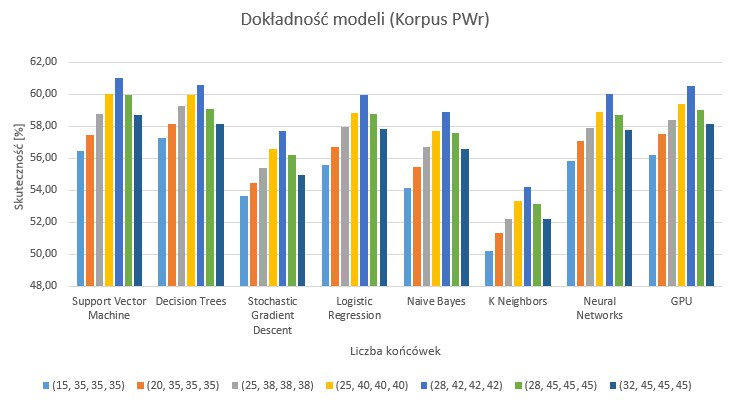
\includegraphics[width=\linewidth]{charts/korpuspwrwykres}
	\label{Rysunek}
	\caption{Skuteczność modeli -- korpus PWr.}
\end{figure}

\begin{figure}[H]
	\centering
	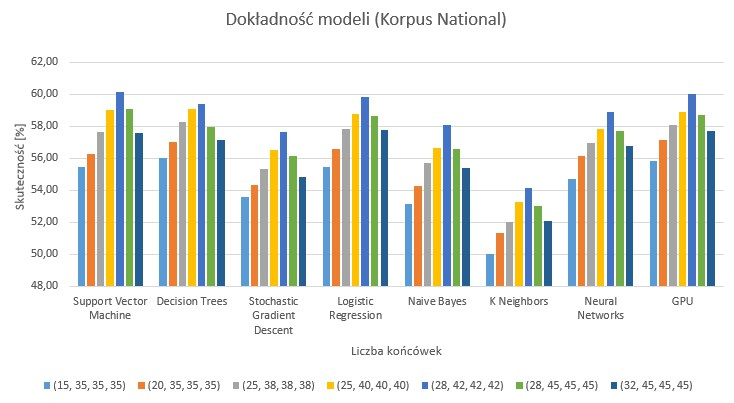
\includegraphics[width=\linewidth]{charts/korpusnationalwykres}
	\label{Rysunek}
	\caption{Skuteczność modeli -- korpus National.}
\end{figure}

\newpage
\subsection{Pomiary czasów uczenia}

\begin{table}[H]
	\centering
	\caption{Pomiary czasów uczenia.}
	\smallskip
	\begin{tabular}{lcc}
		\toprule
		\textbf{Algorytm} & \textbf{Korpus uczący PWr (h:m:s)} &  \textbf{Korpus uczący National (h:m:s)} \\
		\midrule
		Support Vector Machine & 0:44:52 & 23:29:53 \\
		Decision Trees & 0:01:22 & 0:05:48 \\
		Stochastic Gradient Descent & 0:01:20 & 0:04:56 \\
		Logistic Regression & 0:01:32 & 0:07:10 \\
		Naive Bayes & 0:01:18 & 0:04:32 \\
		K Neighbors & 0:01:18 & 0:05:20 \\
		Neural Networks & 0:20:28 & 1:21:04 \\
		GPU Classifier & 0:14:55 & --- \\
		\bottomrule
	\end{tabular}
\end{table}
Do testów został użyty procesor Intel(R) Core(TM) i7-4930K CPU @ 3.40GHz. Jest to wydajna jednostka z 2013 roku pracująca na 6 rdzeniach w technologi Hyper-Threading (12 wątków).
W przypadku klasyfikatora opartego na GPU została wykorzystana karta graficzna NVIDIA GeForce GT 740 (chip GK107) -- model z średniej półki z 2014 roku.
W testach każdy algorytm korzystał z jednego wątku procesora.

Uczenie algorytmów: drzew decyzyjnych, stochastycznego spadku gradientu, regresji logistycznej, naiwnego klasyfikatora bayesowskiego oraz $k$-najbliższych sąsiadów zakończyło się na korpusie uczącym PWr w niewiele ponad minutę. Daje to możliwość wielokrotnego zmieniania parametrów tych algorytmów w poszukiwaniu lepszych wyników. Uczenie sieci neuronowych trwało zdecydowanie dłużej od wcześniej wymienionych, natomiast maszyny wektorów nośnych okazały się prawdziwnym wyzwaniem dla procesora w postaci wielogodzinnych obliczeń modelu danych. Uczenie klasyfikatorów za pomocą korpusu National, ze względu na wielkość danych uczących, jest kilka razy bardziej czasochłonne w porównaniu do korpusu PWr.

\subsection{Pomiary czasów klasyfikacji}

Pomiary czasów klasyfikacji przeprowadzono na próbie 14 zbiorów tekstów zawierających kolejno od 10 do 100 wyrazów z przeskokiem co 10, oraz większe rozmiary: 250, 500, 1000, 2000. Wyniki rozdzielono na osobne grupy przedstawiające odpowiednio klasyfikatory nauczone na korpusie PWr oraz na korpusie podmilionowym.

\newpage

\begin{landscape}
	\begin{table}[H]
		\centering
		\caption{Czasy klasyfikacji w zależności od ilości słów w tekście -- Korpus PWr.}
		\scalebox{.95}{
		\begin{tabular}{ccccccccccccccc}
			\toprule
			\textbf{Algorytm} & \textbf{10} & \textbf{20} & \textbf{30} & \textbf{40} & \textbf{50} & \textbf{60} & \textbf{70} & \textbf{80} & \textbf{90} & \textbf{100} & \textbf{250} & \textbf{500} & \textbf{1000} & \textbf{2000} \\
			\midrule
            Logistic Regression & 0.0076 & 0.0081 & 0.0114 & 0.0154 & 0.0185 & 0.0215 & 0.0242 & 0.0280 & 0.0305 & 0.0340 & 0.0790 & 0.1580 & 0.3160 & 0.4736 \\
			Stochastic Gradient Descent & 0.0030 & 0.0064 & 0.0097 & 0.0140 & 0.0171 & 0.0205 & 0.0232 & 0.0268 & 0.0301 & 0.0336 & 0.0803 & 0.1611 & 0.3206 & 0.4812 \\
			Decision Trees & 0.0039 & 0.0078 & 0.0123 & 0.0167 & 0.0203 & 0.0244 & 0.0277 & 0.0319 & 0.0359 & 0.0399 & 0.0953 & 0.1909 & 0.3814 & 0.5734 \\
			Naive Bayes & 0.0046 & 0.0097 & 0.0148 & 0.0210 & 0.0259 & 0.0310 & 0.0355 & 0.0408 & 0.0458 & 0.0509 & 0.1225 & 0.2460 & 0.4902 & 0.7358 \\
			Neural Networks & 0.3552 & 0.0157 & 0.0244 & 0.0329 & 0.0408 & 0.0484 & 0.0564 & 0.0647 & 0.0729 & 0.0815 & 0.4051 & 0.3911 & 0.7834 & 1.1736 \\
			K Neighbors & 0.0980 & 0.2192 & 0.3260 & 0.4340 & 0.5545 & 0.6481 & 0.7756 & 0.9020 & 1.0012 & 1.1103 & 2.8379 & 5.6259 & 11.2033 & 16.8673 \\
			Support Vector Machine & 0.4625 & 0.7471 & 1.1418 & 1.5333 & 1.9311 & 2.2751 & 2.7042 & 3.1116 & 3.4938 & 3.8904 & 4.1399 & 8.2825 & 16.5498 & 24.7921 \\
			Klasyfikator GPU & 2.2735 & 2.1504 & 3.3241 & 4.5460 & 5.4218 & 6.3891 & 7.6431 & 8.7503 & 10.2526 & 10.9616 & 24.4249 & 52.6103 & 104.2419 & 209.9426 \\
			\bottomrule
		\end{tabular}}
	\end{table}
	
	\begin{table}[H]
		\centering
		\caption{Czasy klasyfikacji w zależności od ilości słów w tekście -- korpus National.}
		\scalebox{.95}{
		\begin{tabular}{ccccccccccccccc}
			\toprule
			\textbf{Algorytm} & \textbf{10} & \textbf{20} & \textbf{30} & \textbf{40} & \textbf{50} & \textbf{60} & \textbf{70} & \textbf{80} & \textbf{90} & \textbf{100} & \textbf{250} & \textbf{500} & \textbf{1000} & \textbf{2000} \\
			\midrule
			Logistic Regression & 0.0062 & 0.0095 & 0.0129 & 0.0165 & 0.0194 & 0.0223 & 0.0255 & 0.0292 & 0.0322 & 0.0353 & 0.0789 & 0.1582 & 0.3156 & 0.4743 \\
			Stochastic Gradient Descent & 0.0031 & 0.0063 & 0.0096 & 0.0136 & 0.0164 & 0.0194 & 0.0225 & 0.0264 & 0.0293 & 0.0328 & 0.0803 & 0.1609 & 0.3202 & 0.4816 \\
			Decision Trees & 0.0039 & 0.0075 & 0.0115 & 0.0161 & 0.0195 & 0.0231 & 0.0270 & 0.0314 & 0.0350 & 0.0389 & 0.0958 & 0.1920 & 0.3817 & 0.5743 \\
			Naive Bayes & 0.0047 & 0.0096 & 0.0146 & 0.0203 & 0.0249 & 0.0294 & 0.0345 & 0.0401 & 0.0447 & 0.0498 & 0.1224 & 0.2456 & 0.4895 & 0.7369 \\
			Neural Networks & 0.0835 & 0.0156 & 0.0236 & 0.0322 & 0.0399 & 0.0471 & 0.0556 & 0.0640 & 0.0718 & 0.0797 & 0.2682 & 0.3896 & 0.7777 & 1.1690 \\
			K Neighbors & 0.4112 & 0.8940 & 1.3225 & 1.7856 & 2.2718 & 2.6559 & 3.1993 & 3.7022 & 4.2142 & 4.6087 & 12.9492 & 25.2313 & 50.9364 & 77.4012 \\
			Support Vector Machine & 0.9388 & 2.0124 & 3.0720 & 4.1224 & 5.1977 & 6.1370 & 7.3113 & 8.3830 & 9.4158 & 10.4554 & 13.7190 & 27.3826 & 54.6263 & 81.9051 \\
			\bottomrule
		\end{tabular}}
	\end{table}
\end{landscape}

Można zauważyć, że najdłuższym czasem klasyfikacji wyróżnił się ten wykorzystujący kartę graficzną, osiągając przy liczbie 2000 wyrazów bardzo długi czas 209,9 s. Lepszy czas osiągnął algorytm \texttt{SVM}, osiągając dla tej samej liczby wyrazów 24,8 s. Trzecim, stosunkowo podobnym do poprzedniego okazał się algorytm \texttt{K Neighbors} -- 16,9 s. Reszta algorytmów może się pochwalić bardzo niskimi i zbliżonymi do siebie czasami.

Faktem również jest, że dla pierwszych pięciu algorytmów, które osiągnęły najlepsze czasy (\texttt{Logistic Regression}, \texttt{SGD}, \texttt{Decision Trees}, \texttt{Naive Bayes}, \texttt{Neural Networks}) czasy klasyfikacji dla korpusu PWr są bardzo zbliżone do czasów klasyfikacji na korpusie podmilionowym. Dla najgorszych algorytmów, czasy klasyfikacji na korpusie podmilionowym są kilkukrotnie wyższe.

Poniższy wykres przestawia wyniki z korpusu PWr. W celu lepszego zobrazowania zależności zostały na nim przedstawione wyniki od 10 do 100 wyrazów. Najszybsze algorytmy osiągnęły czasu rzędu setnych sekundy, dlatego też są prawie niewidoczne na wykresie.

\begin{figure}[H]
	\centering
	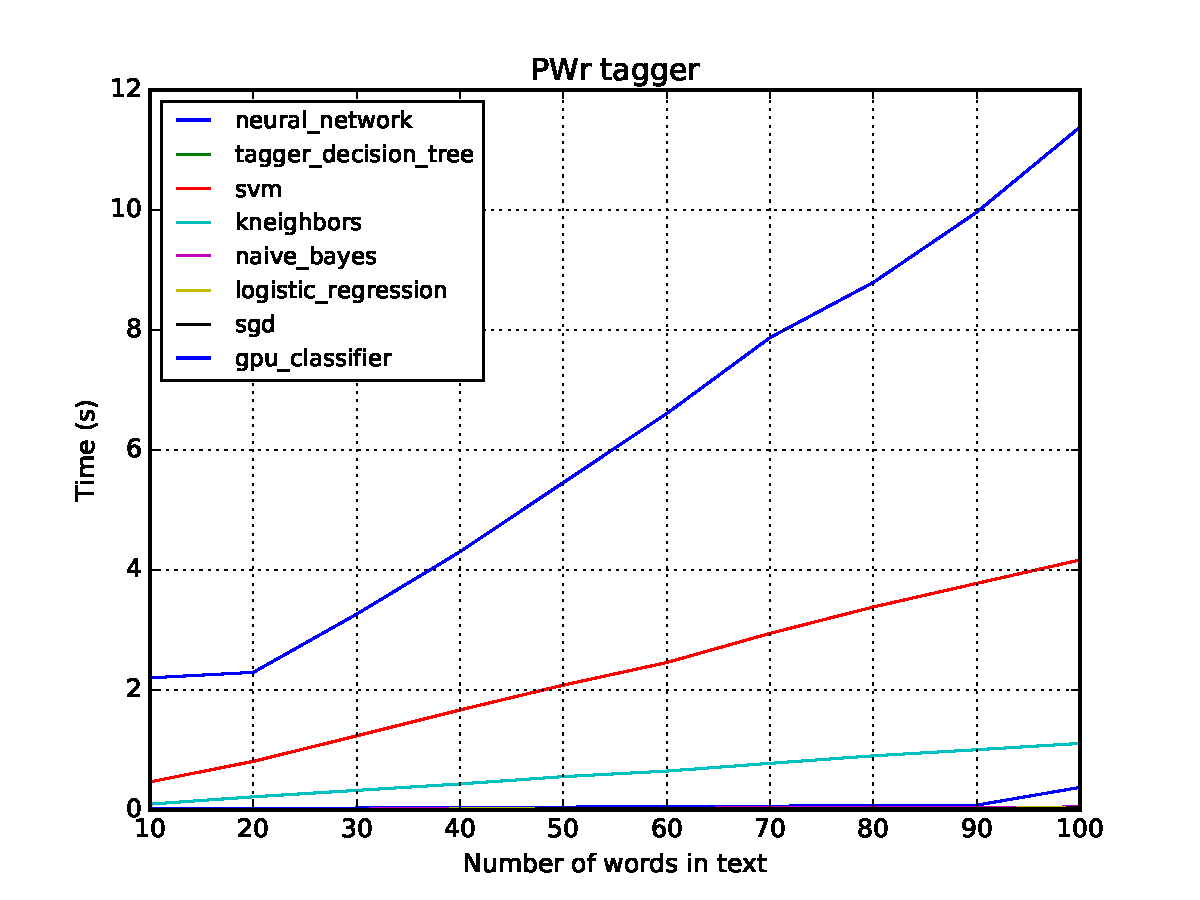
\includegraphics[width=\linewidth]{charts/czasy_pwr.pdf}
	\label{Rysunek}
	\caption{Czasy klasyfikacji w zależności od ilości słów w tekście -- korpus PWr.}
\end{figure}

\newpage

W przypadku korpusu podmilionowego sytuacja jest bardzo podobna z tą różnicą, iż pominięty został algorytm bazujący na karcie graficznej albowiem nie można go było uruchomić na udostępnionej maszynie testowej z powodu niewystarczającej ilości pamięci operacyjnej.

\begin{figure}[H]
	\centering
	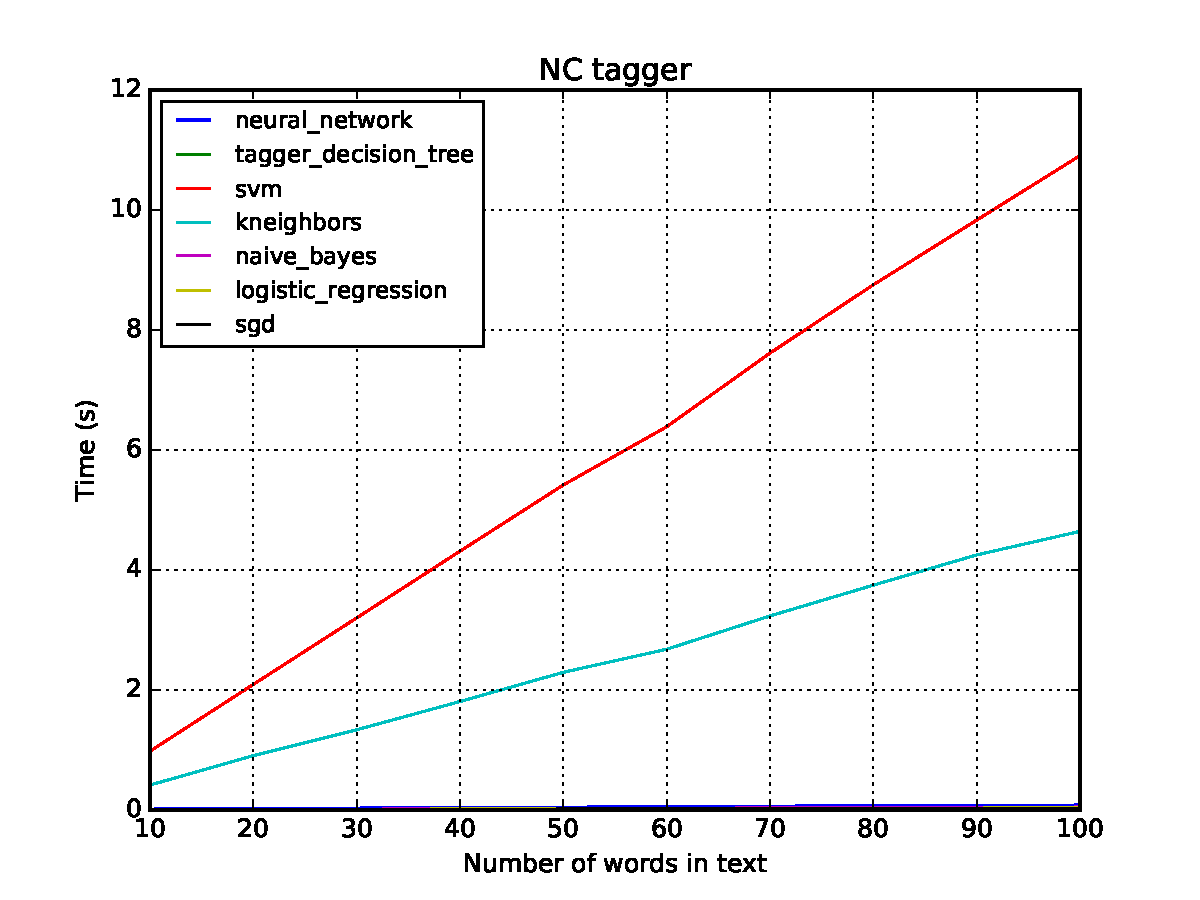
\includegraphics[width=\linewidth]{charts/czasy_nc.pdf}
	\label{Rysunek}
	\caption{Czasy klasyfikacji w zależności od ilości słów w tekście -- korpus National.}
\end{figure}
